\message{ !name(1-recurrence.tex)}\documentclass[addpoints]{exam}
\usepackage{url}
\usepackage{amsmath,amsthm,enumitem}
\usepackage{graphicx}
\usepackage{tikz}
\usepackage{cancel}
\usepackage{float}
\usepackage{caption}
\usepackage{soul}
\usetikzlibrary{positioning}
\tikzset{main node/.style={circle,fill=blue!20,draw,minimum size=1cm,inner sep=0pt},
            }
\def\checkmark{\tikz\fill[scale=0.4](0,.35) -- (.25,0) -- (1,.7) -- (.25,.15) -- cycle;} 
\def\cov{\mathrm{Cov}}
\newcommand{\Exval}[1]{\left< #1\right>}
\newcommand{\ExvalDef}[1]{\sum_{i=0}^{\infty} #1P\left( #1\right)}
\newcommand{\Var}[1]{\sigma^{2}\left( #1\right)}
\newcommand{\VarDef}[1]{\left< #1^{2}\right> - \left< #1\right>^{2}}
\newcommand{\BigO}[1]{\mathcal{O}\left( #1\right)}
\newcommand{\BigT}[1]{\Theta\left( #1\right)}
\newcommand{\BigOmega}[1]{\Omega\left( #1\right)}
\newcommand{\T}[1]{T\left( #1\right)}
\renewcommand{\P}[1]{\left( #1\right)}
\newcommand{\floor}[1]{\lfloor #1\rfloor}
\newcommand{\ceil}[1]{\lceil #1\rceil}
\newcommand{\Lim}[1]{\raisebox{0.5ex}{\scalebox{0.8}{$\displaystyle \lim_{#1}\;$}}}


%\newcommand{\Cov}{\mathrm{Cov}}$


\newcommand{\var}{\text{Var}}
\newtheorem*{claim}{Claim}
\title{CS 6150: A refresher}
\author{Christopher Mertin\\ {\small (Worked with Milinda Fernando)}}
\date{Due Date: Sep 8, 2015}
\begin{document}

\message{ !name(1-recurrence.tex) !offset(-3) }

\maketitle
\begin{center}
\fbox{\fbox{\parbox{5.5in}{\centering
This assignment has \numquestions\ questions, for a total of \numpoints\
points. 
Unless otherwise specified, complete and reasoned arguments will be expected for all answers. }}}
\end{center}

\qformat{Question \thequestion: \thequestiontitle\dotfill \textbf{[\totalpoints]}}
\pointname{}
\bonuspointname{}
\pointformat{[\bfseries\thepoints]}

\printanswers

\begin{center}
  \gradetable
\end{center}
\newpage

\begin{questions}

\titledquestion{Recurrences I}

Solve each of the following recurrences. You may use any method you like, but please show your work. In each recurrence, you may assume convenient starting values for $T(0)$ or $T(1)$ unless otherwise specified.. Note that $c$ is an undetermined constant. 

Solving a recurrence means that you provide a bound of the form $T(n) = O(f(n))$ for a specific $f$. Tight bounds get full credit: for example, if the recurrence is $T(n) = 2T(n/2) + cn$, the answer $T(n) = O(n^2)$ is correct but not precise enough, and you will not get full credit for it. 

\begin{parts}
\part[2] $T(n) = 7T(n/2) + cn^2$
\begin{solution}
%\EvalDef{j}\\
\begin{align}
\intertext{This solution uses the first case of the Master's Theorem}
\log_{2}(7) &\approx 2.81\\
\intertext{Since $n^{\log_{2}(7)} > f(n)$}
\Rightarrow n^{2.81} &> cn^{2}\\
T(n) &= \BigT{n^{\log_{2}(7)}}
\end{align}
\end{solution}

\part[2] $T(n) = 3T(n/2) + cn$
\begin{solution}
\begin{align}
\intertext{This solution uses the first case of the Master's Theorem}
\log_{2}(3) &= 1.58\\
\intertext{Since $n^{1.58} > f(n)$}
\Rightarrow n^{1.58} &= cn\\
T(n) &= \BigT{n^{log_{2}(3)}}
\end{align}
\end{solution}

\part[2] $T(n) = T(n/5) + c$
\begin{solution}
\begin{align}
\intertext{This solution uses the second case of the Master's Theorem}
\log_{5}(1) = 0\\
\intertext{Since $n^{c} = n^{\log_{b}(a)}$}
\Rightarrow n^{0} &= n^{0}\\
T(n) &= \BigT{\log(n)}
\end{align}
\end{solution}

\part[2] $T(n) = T(n/2) + T(3n/10) + cn$
\begin{solution}
\begin{align}
\intertext{Longest path on recursion tree:}
\frac{n}{2^{i}} &= 1\\
i &= \log_{2}(n)
\intertext{From the recursion tree, guess $n\log(n)$ from there being $\log(n)$ terms of $n$ at
the longest recursion path}
T(n) &\leq \T{\frac{n}{2}} + \T{\frac{3n}{10}} + cn\\
T(n) &\leq c\P{\frac{n}{2}}\log\P{\frac{n}{2}} + c\P{\frac{3n}{10}}\log\P{\frac{3n}{10}} + cn\\
T(n) &\leq \left[ c_{1}\P{\frac{n}{2}}\P{\log(n)-\log(2)}+\P{c_{2}\P{\frac{3n}{10}}}\P{\log(3n)-\log(10)}\right] + cn\\
T(n) &\leq \left[ c_{1}nlog(n) + c_{2}\right] + \left[ c_{3}nlog(3n)+c_{4}\right] + c_{5}n\\
T(n) &\leq c_{1}nlog(n) + c_{2}nlog(3n) + c_{3}n + c_{4}\\
T(n) &\leq \BigO{n\log(n)}\checkmark
\end{align}
\end{solution}

\part[2] $T(n) = 2T(n-1) + 10n^2$
\begin{solution}
\begin{align}
&T(n-1) = 2T(n-2) + 10(n-1)^{2}\\
T(n) &= 2\left[2T(n-2) + 10(n-1)^{2}\right] + 10n^{2}\\
T(n) &= 2^{2}T(n-2) + 2\cdot 10(n-1)^{2} + 10n^{2}\\
&T(n-2) = 2T(n-3) + 10(n-2)^{2}\\
T(n) &= 2^{2}\left[2T(n-3)+10(n-2)^{2}\right]+2\cdot 10(n-1)^{2}+10n^{2}\\
T(n) &= 2^{3}T(n-3)+10\left[ 2^{2}(n-2)^{2}+2(n-1)^{2}+n^{2}\right]\\
\vdots\nonumber\\
T(n-k) &= 2^{k+1}T(n-k) + 10\sum_{i=0}^{k}2^{k}(n-k)^{i}\\
T(n) &= \BigO{2^{n}}
\end{align}
\end{solution}
\end{parts}


\titledquestion{Recurrences II}

Solve each of the following recurrences. The same note as above applies here. 

\begin{parts}
\part[3] $T(n) = T(n-1) T(n-2)$ (hint: you can express your answer in terms of the $n^{\text{th}}$ Fibonacci number $F(n)$) 
\begin{solution}


\begin{align}
% T(n) &= T(n-1)T(n-2)\\
% &\quad\ T(n-1) = T(n-2)T(n-3)\nonumber\\
% &\quad\ T(n-2) = T(n-3)T(n-4)\nonumber\\
% T(n) &= \left[ T(n-2)T(n-3)\right]\left[ T(n-3)T(n-4)\right] = T(n-2)\left[ T(n-3)\right] ^{2} T(n-4)\\
% &\quad\ T(n-2) = T(n-3)T(n-4)\nonumber\\
% &\quad\ T(n-3) = T(n-4)T(n-5)\nonumber\\
% &\quad\ T(n-4) = T(n-5)T(n-6)\nonumber\\
% T(n) &= T(n-3)T(n-4)\left[ T(n-4)T(n-5)\right]^{2}T(n-5)T(n-6)\nonumber\\
%      &= T(n-3)\left[ T(n-4)\right]^{3}\left[ T(n-5)\right]^{3}T(n-6)\\
% &\quad\ T(n-3) = T(n-4)T(n-5)\nonumber\\
% &\quad\ T(n-4) = T(n-5)T(n-6)\nonumber\\
% &\quad\ T(n-5) = T(n-6)T(n-7)\nonumber\\
% &\quad\ T(n-6) = T(n-7)T(n-8)\nonumber\\
% T(n) &= T(n-4)\left[ T(n-5)\right] ^{4}\left[ T(n-6)\right]^{6}\left[T(n-7)\right]^{4}T(n-8)\\
% &\quad\ T(n-4) = T(n-5)T(n-6)\nonumber\\
% &\quad\ T(n-5) = T(n-6)T(n-7)\nonumber\\
% &\quad\ T(n-6) = T(n-7)T(n-8)\nonumber\\
% &\quad\ T(n-7) = T(n-8)T(n-9)\nonumber\\
% &\quad\ T(n-8) = T(n-9)T(n-10)\nonumber\\
% T(n) &= T(n-5)\left[ T(n-6)\right]^{5}\left[ T(n-7)\right]^{10}\left[ T(n-8)\right]^{10}\left[ T(n-9)\right]^{5}T(n-10)\\
% \intertext{The powers of the recurrences are every line of Pascal's Triangle, thus the $k^{th}$ iteration would be as follows:}
% T(n) &= \prod_{i=0}^{k}T(n-k-i)^{k \choose i};\quad {k \choose i} = \frac{k!}{i!(k-i)!};\quad k\geq 1\\
% \intertext{The recurrence that is going to take the most time is going to be in the center of the sequence, which will be the $\floor{\frac{k}{2}}\ k^{th}$ term. {\color{red} Quite possibly can lower bound with using the $k^{th}$ term with $\Omega$ and maybe upperbound somehow???}}
\intertext{We can take the logarithm of both sides of the original time complexity, resulting in}
\log\P{T(n)} &= \log\P{T(n-1)T(n-2)} = \log\P{T(n-1)} + \log\P{T(n-2)}\\
\intertext{As stated in the question, the $n^{th}$ Fibonacci number can be represented by $F(n)$. We can see that the logarithm of a time complexity is equal to that Fibonacci number as it would be the height of the recursive portion of the tree. This is why this conversion can be made. By doing so, we get the equation of the Fibonacci sequence:}
F(n) &= F(n-1) + F(n-2)
This is some text
\end{align}
\end{solution}

\part[3] $T(n) = n^{2/3}T(\sqrt{n}) + n^{1.2}$
\begin{solution}
\emph{Solutions are hard}
\end{solution}
\part[3] $T(n) = T(n-3) + 8^n$
\begin{solution}
\begin{align}
\intertext{Creating a recurion tree, it will stop at $8^{n}-\left( 8^{n}+3\right)$, where this can be used to find the height of the recurion tree by:}
8^{n}+3 &= 3^{i}\\
i &= \log_{3}\left(8^{n}+3\right)
\intertext{From this, we can change the time complexity to be:}
T(n) &= \sum_{i=0}^{\log_{3}\left( 8^{n}+3\right)}8^{n}-3^{i}\\
T(n) &= 8^{n}-\underbrace{\sum_{i=0}^{\log_{3}\left( 8^{n}+3\right)}3^{i}}_{\text{Geometric Series}}\\
&\quad \sum_{i=0}^{\log_{3}\left( 8^{n}+3\right)}3^{i} = \frac{3^{\log_{3}\left( 8^{n}+3\right) +1}-1}{1-3}\\
&\quad \phantom{\ \sum_{i=0}^{\log_{3}\left( 8^{n}+3\right)}3^{i} } = \frac{3\left( 8^{n}+3\right) -1}{-2} = \frac{1-3\cdot 8^{n}+9}{2}\\
T(n) &= 8^{n} - \frac{1}{2} + \frac{3}{2}8^{n}-9\\
T(n) &= \frac{5}{2}8^{n}-\frac{19}{2}\\
T(n) &= \BigO{8^{n}}
\end{align}
\end{solution}

\part[3] $T(n) = \sum_{k = 0}^{n-1} (k \cdot T(k-1))$, where $T(0) = 1$. 
\begin{solution}
\emph{Omitted by Dr. Suresh Venkatasubramanian}
\end{solution}

\part[3] $T(n) = n +  \sum_{i = 1}^{\log n} T(n/2^i)$.
\begin{solution}
\begin{align}
\intertext{From the recursion tree, we can solve for the height of it to be:}
\frac{n}{2^{i}} &= 1\\
i &= \log_{2}(n)
%\intertext{We can thus rearrange the time complexity to be:}
%T(n) &= n + \sum_{i=1}^{\log(n)}T\P{\frac{n}{2^{i}}} = n + T\P{\frac{n}{2}} + T\P{\frac{n}{2^{2}}} + \dotsm + T\P{\frac{n}{2^{\log(n)}}}
\intertext{As there is only one thing going on in this recursion, we can sum the time complexity recursion tree to get the closed form of the solution. From the recursion tree:}
T(n) &= n+\frac{n}{2}+\frac{n}{4}+\dotsm +1\\
T(n) &= n\sum_{i=0}^{m-1}\P{\frac{1}{2}}^{i} = n\frac{1-\P{\frac{1}{2}}^{n}}{\frac{1}{2}} = 2\left[ n-\P{\frac{1}{2}}^{n}n\right]\\
\intertext{Therefore, the sum total is:}
T(n) &= \log(n)\left[2n-\P{\frac{1}{2}}^{n}n\right]
\intertext{Which reduces to the following since $\Lim{n\rightarrow \infty}\P{\frac{1}{2}}^{n}n=0$}
T(n) &= \BigO{n\log(n)}
\end{align}
\end{solution}
\end{parts}

\titledquestion{Probability I}
\begin{parts}
  \part[2] \texttt{d10} is a decahedron die used in Dungeons and Dragons with
  the ten faces labeled with the numbers $1$ through $10$. What is the expected
  value of a roll? What is the variance?
\begin{solution}
\begin{align}
\Exval{X} &= \ExvalDef{x}\\
\intertext{Probability of any roll is $\frac{1}{10}$}
\Exval{X} &= \frac{1}{10}\left( \sum_{x=1}^{10}x\right) = \frac{55}{10} = 5.5\\
\Exval{X^{2}} &= \frac{1}{10}\left( \sum_{x=1}^{10}x^{2}\right) = \frac{385}{10} = 38.5\\
\intertext{The variance is defined by:}
\Var{X} &= \VarDef{X} = 38.5 - 30.25 = 8.25
\end{align}
\end{solution}

\part[2] Show that $\binom{n}{k} \le n^k/k!$. Using Stirling's approximation for
the factorial function
\[ n! \simeq \left(\frac{n}{e}\right)^n \sqrt{2\pi n} \]
show that $\binom{n}{k} \simeq \P{\frac{ne}{k}}^k$
\begin{solution}
\begin{itemize}
\item Show that $\binom{n}{k} \le n^k/k!$
\end{itemize}
\begin{align}
{n \choose k} &= \frac{n!}{k!(n-k)!}\\
\intertext{\underline{For $n=k$}}
\frac{\cancel{n!}}{\cancel{n!}(0)!} &= 1 < \frac{n^{k}}{k!}\checkmark\\
\intertext{\underline{For $n>k$}}
\frac{n\cdot (n-1)\dotsm (n-k+1)\cancel{(n-k)!}}{k!\cancel{(n-k)!}} &= \frac{n\cdot (n-1)\dotsm (n-k+1)}{k!} < \frac{n^{k}}{k!}\ \checkmark
\end{align}

\begin{itemize}
\item Using Stirling's approximation for
the factorial function
\[ n! \simeq \left(\frac{n}{e}\right)^n \sqrt{2\pi n} \]
show that $\binom{n}{k} \simeq \P{\frac{ne}{k}}^k$
\begin{align}
\intertext{The problem seems ill-posed as there is no way to actually get ${n \choose k}\simeq \P{\frac{ne}{k}}^k$, but what we can do is show that they are approximately in the same order of magnitude by calculating a lower bound and upper bound.}
\intertext{\begin{center}\underline{Upper Bound}\end{center}}
{n \choose k} &= \frac{n!}{k!(n-k)!} \approx \frac{n!e^{k}}{(n-k)!k^{k}\sqrt{2\pi k}}\\
\intertext{Since $n!\leq n^{k}$}
\frac{n!e^{k}}{(n-k)!k^{k}\sqrt{2\pi k}} &\leq \frac{n^{k}e^{k}}{(n-k)!k^{k}\sqrt{2\pi k}} \leq \P{\frac{ne}{k}}^{k} \checkmark
\intertext{\begin{center}\underline{Lower Bound}\end{center}}
{n \choose k} = \frac{n!}{k!(n-k)!} &\geq \frac{n!}{k^{k}n^{k}} \geq \frac{n^{n}\sqrt{2\pi n}}{e^{n}k^{k}n^{k}} \geq \frac{n^{n-k}}{e^{n}k^{k}}\ \checkmark
\intertext{Therefore, we can say that $\frac{n^{n-k}}{e^{n}k^{k}} \leq {n \choose k} \leq \P{\frac{ne}{k}}^{k}\ \checkmark$}
\end{align}
\end{itemize}


% \begin{itemize}
% \item 
% \begin{align}
% \end{align}
% \end{itemize}




\end{solution}
\part[2] Use a Taylor expansion to justify the approximation
\[ e^{-x} \simeq 1-x \]
for $x$ near $0$. 
\begin{solution}
\begin{align}
\intertext{The definiton of the Taylor Series Expansion about some point $a$ is:}
\sum_{n=0}^{\infty}&\frac{f^{(n)}(a)}{n!}(x-a)^{n}\\
\intertext{with $f^{(n)}(a)$ being the $n^{th}$ derivative of $f(a)$. Taking the Taylor Series expansion of $e^{-x}$ results in:}
f(a) &= e^{-a}\\
f^{(0)}(a) &= \left.\frac{e^{-a}}{0!}(x-a)^{0}\right|_{a=0}=1\\
f^{(1)}(a) &= -\left.\frac{e^{-a}}{1!}(x-a)^{1}\right|_{a=0}=-x\\
f^{(2)}(a) &= \BigO{x^{2}}\\
\intertext{Therefore, the first-order approximation of $e^{-x}$ about $x=0$ is}
e^{-x} &= 1-x+\BigO{x^{2}} \simeq 1-x
\end{align}
\end{solution}

\part[4] A set of random variables $X_1, X_2, \ldots, X_k$ is said to be
\emph{mutually independent} if for any subset $S = \{j_1, j_2, \ldots, j_k\} \subset \{1, 2, \ldots, k\}$
it holds that 
\[ \Pr(X_{j_1} = v_i, X_{j_2} = v_2, \ldots, X_{j_k} = v_k) = \prod_i
\Pr(X_{j_i} = v_i)\]
The same set of random variables is said to be \emph{pairwise independent} if
this holds for subsets of size $k = 2$, but not necessarily for larger
subsets. Construct a set of three variables that are \emph{not} mutually
independent but are pairwise independent.
\begin{solution}
\begin{align}
\intertext{To rephrase what this is asking for:}
P\P{x_{1}\cap x_{2} \cap x_{3}} &\neq P\P{x_{1}}\cdot P\P{x_{2}}\cdot P\P{x_{3}}
\intertext{but...}
P\P{x_{1}\cap x_{2}} &= P\P{x_{1}}\cdot P\P{x_{2}}\\
P\P{x_{1}\cap x_{3}} &= P\P{x_{1}}\cdot P\P{x_{3}}\\
P\P{x_{2}\cap x_{3}} &= P\P{x_{2}}\cdot P\P{x_{3}}
\end{align}
\begin{table}[H]
\centering
\caption*{\vspace{-1em}Values}
\begin{tabular}{@{}l | c | r@{}}
  \hline\hline
  $x_{1}$ & $x_{2}$ & $x_{3}$\\
  \hline
  0 & 0 & 0\\
  1 & 0 & 1\\
  0 & 1 & 1\\
  1 & 1 & 0\\
  \hline\hline
\end{tabular}
\end{table}
Each combination has a probability of $\frac{1}{4}$ succeeding in producing 1, meaning this fits the defintion from above.
\end{solution}

\end{parts}
\titledquestion{Probability II}
\begin{parts}
  \part[4] A strange clause in a version of Dungeons and Dragons says: roll a
  \texttt{d6} (a six-sided die with faces from $1$ to $6$). If the value rolled
  is $3$ or less, roll a \texttt{d8} else roll a \texttt{d10}. Add the two
  values obtained. 

  Let $X$ be the value of the \texttt{d6} roll and let $Y$ be the value of the
  other die roll. 
  \begin{itemize}
  \item Is it true that $E[X + Y] = E[X] + E[Y]$?
  \item Is it true that $\var(X + Y) = \var(X) + \var(Y)$? 
  \end{itemize}
  Compute the expectation and variance of the overall value obtained.
\begin{solution}
\begin{itemize}
\item \text{Is it true that }$E[X + Y] = E[X] + E[Y]$\text{?}
\begin{align*}
\left< j\right> &= \sum_{j=0}^{\infty}jP(j)\\
\left< X+Y\right> &= \sum_{x=0}^{\infty}\sum_{y=0}^{\infty}P_{XY}\left( x,y\right)\\
                  &= \sum_{x=0}^{\infty}\sum_{y=0}^{\infty}xP_{XY}\left( x,y\right) + \sum_{y=0}^{\infty}\sum_{x=0}^{\infty}yP_{XY}\left( x,y\right)\\
                  &= \sum_{x=0}^{\infty}xP_{X}(x) + \sum_{y=0}^{\infty}yP_{Y}(y)\\
                  &= \left< X\right> + \left< Y\right>\ \checkmark\\
\intertext{From the above it can be said that, yes, it is true that $\Exval{X+Y} = \Exval{X} + \Exval{Y}$}
\left< X\right> &= \sum_{x=1}^{6}\frac{x}{6} = 3.5\\
\left< Y_{1}\right> &= \sum_{y_{1}=1}^{8}\frac{y_{1}}{8} = 4.5\\
\left< Y_{2}\right> &= \sum_{y_{2}=1}^{10}\frac{y_{2}}{10} = 5.5\\
\left< Y\right> &= \frac{1}{2}\left( \left< Y_{1}\right> + \left< Y_{2}\right>\right) = 5.0\\
%\left< X\right> + \left< Y\right> &= 3.5 + 5.0 = 8.5\\
\left< X+Y\right> &= \sum_{x=1}^{6}\frac{x}{6} + \frac{1}{2}\left( \sum_{y_{1}=1}^{8}\frac{y_{1}}{8} + \sum_{y_{2}=1}^{10}\frac{y_{2}}{10}\right) = 3.5 + \frac{1}{2}\left(4.5 + 5.5\right) = 8.5\\
\end{align*}
\end{itemize}
\end{solution} 
%\ \newpage
\begin{solution}
\begin{itemize}
\item \text{Is it true that }$\var (X + Y) = \var (X) + \var (Y)$\text{?}
\begin{align*}
\Var{j} &= \VarDef{j}\\
\left< XY\right> &= \sum_{x=1}^{n}\sum_{y=1}^{n}xyP(x)P(y) = \sum_{x=1}^{n}\left( xP(x)\underbrace{\sum_{y=1}^{n}yP(y)}_{\left< Y\right>}\right)\\ 
&= \left(\left< Y_{1}\right> \sum_{x=1}^{3}xP(x) + \left< Y_{2}\right>\sum_{x=4}^{6}xP(x)\right) \\
&= 4.5(1.0) + 5.5\left(\frac{5}{2}\right) = \frac{73}{4}\\ 
\Exval{X^{2}} &= \sum_{x=1}^{6}\frac{x^{2}}{6} = \frac{91}{6}\\
\Exval{Y^{2}} = \Exval{\left( \frac{1}{2} \left( Y_{1}+Y_{2}\right)\right)^{2}} &= \frac{1}{4}\left( \left< Y_{1}^{2}\right> + \left< Y_{2}^{2}\right> + 2\left< Y_{1}Y_{2}\right> \right)\\
&= \frac{1}{4}\left( \left< Y_{1}^{2}\right> + \left< Y_{2}^{2}\right> + 2\left< Y_{1}\right>\cdot\left< Y_{2}\right> \right)\\
&= \frac{1}{4}\left(  \sum_{y_{1}=1}^{8}\frac{y_{1}^{2}}{8} +  \sum_{y_{2}=1}^{10}\frac{y_{2}^{2}}{10} + 2(4.5)5.5\right) = \frac{227}{8}\\
\left< \left(X + Y\right)^{2}\right> = \left< X^{2} + 2XY + Y^{2}\right> &= \left< X^{2}\right> + 2\left< XY\right> + \left< Y^{2}\right>\\
&= \frac{91}{6} + 2\left(\frac{73}{4}\right) + \frac{227}{8} = \frac{1921}{24}\\
\sigma^{2} \left( X+Y\right) &= \left< \left(X + Y\right)^{2}\right> - \left< X+Y\right>^{2} = \frac{1921}{24} - 8.5^{2} = 7.791\bar{6}\\
\sigma^{2} \left( X\right) &= \left< X^{2}\right> - \left< X\right>^{2} = \frac{91}{6} - 3.5^{2} = 2.91\bar{6}\\
\sigma^{2} \left( Y\right) &= \left< Y^{2}\right> - \left< Y\right>^{2} = \frac{227}{8} - 5.0^{2} = \frac{27}{8}\\
\sigma^{2} (X) + \sigma^{2}(Y) &= 2.91\bar{6} +\frac{27}{8} = 6.291\bar{6}
\intertext{From the above it can be seen that $\Var{X+Y} \neq \Var{X} + \Var{Y}$ since the values are not independent and has the extra
term for the covariance. These would be the same if both of the variables were independent random variables as the covariance would then be zero.}
\end{align*}
\end{itemize}
\end{solution} 
  \part[5] Your favorite game store is constantly sold out of the latest edition
  of the Dungeons and Dragons Monster Guide. In fact, the probability of you
  finding the book when you visit the store is $p$. What is the expected number
  of times you'll need to visit to purchase the guide and continue your DnD
  adventures? 
\begin{solution}
\begin{align}
\intertext{For the game to be there, you want an expectation value of 1. Thus}
\Exval{\text{buy}} &= 1 = \sum_{i=0}^{\infty}d_{i}p
\intertext{As $p$ is independent of the sum, you can divide by it and thus solves for the total number of days}
\sum_{i=0}^{\infty}d_{i} &= \frac{1}{p}
\end{align}
\end{solution}
\end{parts}
\titledquestion{Pigeons and Probability}
\begin{parts}
  \part[2]
  The pigeonhole principle says that if you have $m$ objects and $n < m$ buckets
  to put them in, then at least one bucket contains two objects. Prove that if
  you have a random variable $X$ taking positive integer values such that
  $E[X] = k$, then there must be at least one integer $r > k$ such that
  $\Pr(X = k) > 0$.
\begin{solution}
As this question is basically calculating the average, what it is saying is that for the average to be $k$, there must be some value greater than $k$ with a probability greater than $0$, and it asks us to prove this.
\begin{align}
\intertext{\bf Proof by Contradiction:}
\intertext{Assume there is a value of $r < k$ such that $P(X=r)>0$. Therefore, when calculating $\Exval{X}$}
\Exval{X} &= \frac{\sum_{i=1}^{N}x_{i}}{N} = \frac{x_{1}+x_{2}+\dotsm +x_{N}}{N} = k\\
\intertext{If some value of $x_{i}$ is $r$ which is less than $k$, then the expectation value becomes}
\Exval{X^{\prime}} &= \frac{\sum_{i=1}^{N}x_{i}}{N} = \frac{x_{1}+\dotsm + r + \dotsm + x_{N}}{N}
\intertext{Which, by definition of the expectation value/average, makes it less than $k$. Therefore, for the expectation value to be $k$, there must be some value $r>k$ such that $P(X=r) > 0$.}\end{align}
\end{solution}

  \part[4]
  We can think of the above as a probabilistic proof of existence. We're using
  probabilistic techniques to show that an object (deterministically)
  exists. Let's apply it to a problem.

  Let $G = (V, E)$ be a graph and let $H \subset V$. The \emph{induced subgraph}
  $G[H]$ is the graph with vertex set $H$ and whose edges are all edges of $G$
  whose endpoints are in $H$ (i.e are elements of $H \times H \cap E$). 

  A graph $G = (V, E)$ is \emph{bipartite} if $V$ can be partitioned into two
  sets $A, B$ (note that $A, B$ are disjoint and $A \cup B = V$) such that all
  edges go between $A$ and $B$ (i.e $E \subset A \times B$). 

  Show that any graph $G$ with $m$ edges contains a \st{induced} bipartite subgraph
  with $m/2$ edges (Hint: define a random process such that the desired quantity
  is its expectation). 
\begin{solution}
\underline{Random Process:} \emph{Take a random cut through G}\\
{\bf Proof by Contradition:} Assume that a random cut through $G$ would {\em not} have the possiblity of creating a bipartite subgraph with $\frac{m}{2}$ edges. Thus, consider the following graph with the number of edges labeled as $m$


  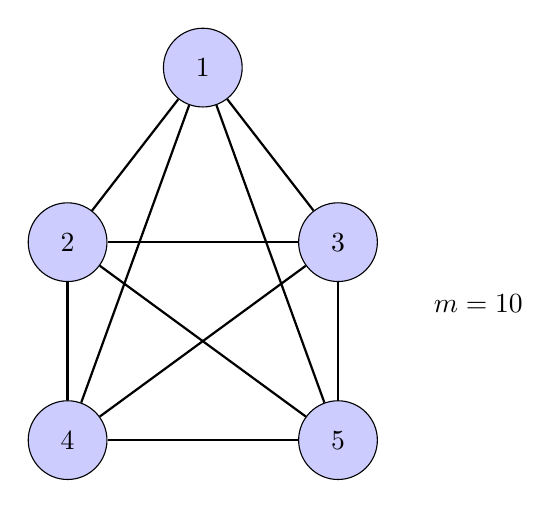
\begin{tikzpicture}
    \node[main node] (1) {$1$};
    \node[main node] (2) [below left = 1.5cm and 1cm of 1]  {$2$};
    \node[main node] (3) [below right = 1.5cm and 1cm of 1] {$3$};
    \node[main node] (4) [below = 1.5cm of 2] {$4$};
    \node[main node] (5) [below = 1.5cm of 3] {$5$};

    \path[draw,thick]
    (1) edge node {} (2)
    (1) edge node {} (5)
    (1) edge node {} (3)
    (1) edge node {} (4)
    (2) edge node {} (5)
    (2) edge node {} (4)
    (2) edge node {} (3)
    (3) edge node {} (4)
    (3) edge node {} (5)
    (4) edge node {} (5);

    \node at (3.5,-3) {$m=10$};
\end{tikzpicture}
\\If this assumption is to hold true, then there shouldn't be any random line $\ell$ that would cause any subgraph with $\frac{m}{2}$ edges to become bipartite. Looking back at the graph above, the requirements would be for any subgraph to be bipartite with only 5 edges. By drawing a random cut through $G$

  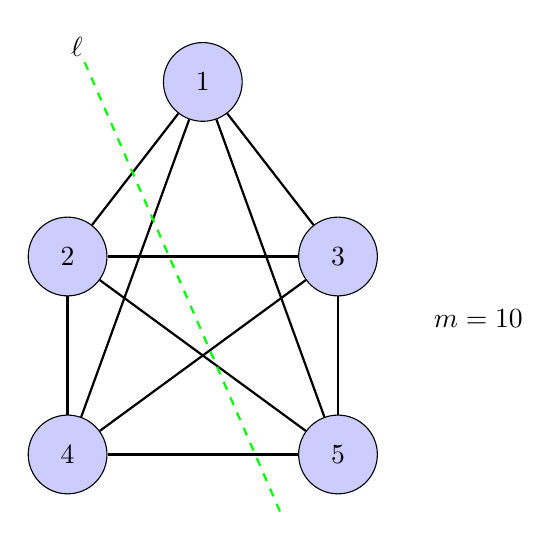
\begin{tikzpicture}
    \node[main node] (1) {$1$};
    \node[main node] (2) [below left = 1.5cm and 1cm of 1]  {$2$};
    \node[main node] (3) [below right = 1.5cm and 1cm of 1] {$3$};
    \node[main node] (4) [below = 1.5cm of 2] {$4$};
    \node[main node] (5) [below = 1.5cm of 3] {$5$};

    \path[draw,thick]
    (1) edge node {} (2)
    (1) edge node {} (5)
    (1) edge node {} (3)
    (1) edge node {} (4)
    (2) edge node {} (5)
    (2) edge node {} (4)
    (2) edge node {} (3)
    (3) edge node {} (4)
    (3) edge node {} (5)
    (4) edge node {} (5);

    \node at (3.5,-3) {$m=10$};

    \draw[dashed,thick,green] (-1.5cm,.25cm) -- (1cm,-5.5cm);
    \node at (-1.6,.45cm) {$\ell$};
\end{tikzpicture}
\\By separating these nodes into two sets and removing extra edges, the graph should be able to be separated into two sets of nodes which are bipartite and subgraphs of $G$


  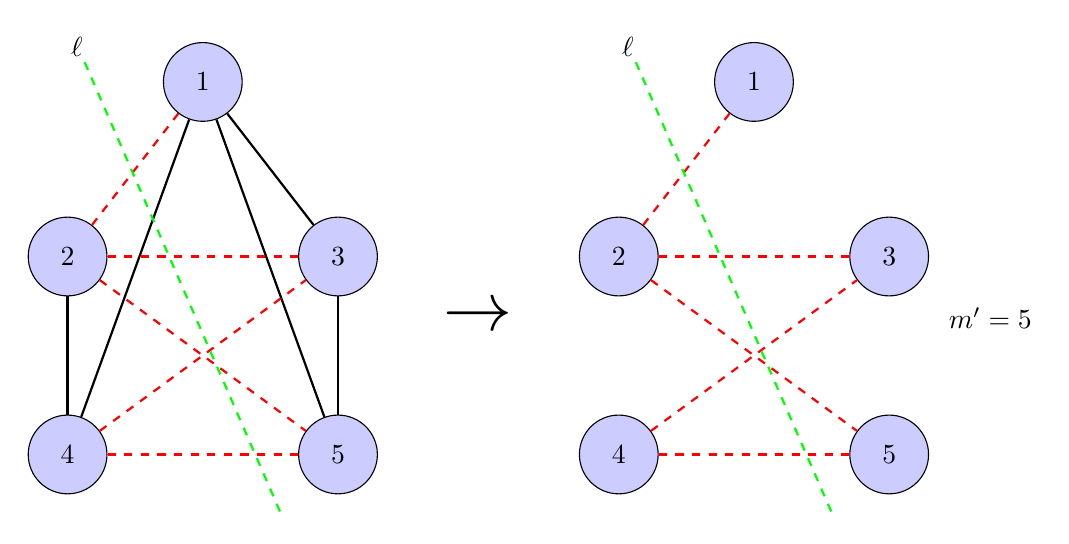
\begin{tikzpicture}
    \node[main node] (1) {$1$};
    \node[main node] (2) [below left = 1.5cm and 1cm of 1]  {$2$};
    \node[main node] (3) [below right = 1.5cm and 1cm of 1] {$3$};
    \node[main node] (4) [below = 1.5cm of 2] {$4$};
    \node[main node] (5) [below = 1.5cm of 3] {$5$};

    \path[draw,thick]
    (1) edge node {} (5)
    (1) edge node {} (3)
    (1) edge node {} (4)
    (2) edge node {} (4)
    (3) edge node {} (5);

    \path[draw,thick,red,dashed]
    (2) edge node {} (1)
    (2) edge node {} (3)
    (2) edge node {} (5)
    (4) edge node {} (5)
    (4) edge node {} (3);

    \draw[dashed,thick,green] (-1.5cm,.25cm) -- (1cm,-5.5cm);
    \node at (-1.6,.45cm) {$\ell$};

    \node at (3.5,-3) {\Huge$\rightarrow$};
    \begin{scope}[xshift=7cm]
      \node[main node] (1) {$1$};
      \node[main node] (2) [below left = 1.5cm and 1cm of 1]  {$2$};
      \node[main node] (3) [below right = 1.5cm and 1cm of 1] {$3$};
      \node[main node] (4) [below = 1.5cm of 2] {$4$};
      \node[main node] (5) [below = 1.5cm of 3] {$5$};
      \node at (3cm,-3cm) {$m^{\prime}=5$};

    \path[draw,thick,red,dashed]
    (2) edge node {} (1)
    (2) edge node {} (3)
    (2) edge node {} (5)
    (4) edge node {} (5)
    (4) edge node {} (3);

    \draw[dashed,thick,green] (-1.5cm,.25cm) -- (1cm,-5.5cm);
    \node at (-1.6,.45cm) {$\ell$};
    \end{scope}
\end{tikzpicture}
\\By removing the edges in $G$ except for those that contain the subgraph that was decided by the random cut $\ell$, it is easy to see that this graph contains a bipartite subgraph due to the random cut from $\ell$. It is bipartite because the nodes $\left\{ 2,4\right\}$ are not connected and the nodes $\left\{ 1,3,5\right\}$ are not connected. Therefore, by proof of contradiction, a random cut will produce a bipartite graph in any given graph.
\end{solution}
  \end{parts}
\end{questions}
\end{document}

\message{ !name(1-recurrence.tex) !offset(-548) }
